\section{Symetrické šifry}
\hyphenation{AES-NI}
Šifra s tajným klíčem je taková, u které se pro šifrování i dešifrování zprávy používá téměř stejný tajný klíč. Bezpečnost a integrita dat u těchto šifer je dána tím, že příslušný klíč je znám pouze oprávněným stranám \parencite{tesar2021}.

Jedním z nejznámějších systémů založených na symetrické kryptografii jsou šifry zpracovávající data po blocích. Standard AES (\enquote{Advanced Encryption Standard}) není bloková šifra, jak je často ve veřejných publikacích uváděno. Jedná se totiž o standard, vydaný americkým institutem NIST (National Institute of Standards and Technology), který využívá symetrickou blokovou šifru pod názvem Rijndael. Algoritmus provádí několik předem definovaných cyklů (rund), během nichž dochází k substitucím a permutacím s jedním klíčem. Princip jednotlivých etap je složitý na popis a je podstatný pouze pro ty, kteří algoritmus implementují do svého systému \parencite{nist2023}.

V praxi se AES nejčastěji využívá k šifrování disků nebo zabezpečení síťové komunikace. Pro urychlení výpočtu tohoto algoritmu byly od roku 2010 zavedeny speciální instrukce do procesorů, například Intel\textregistered{} AES-NI, které jsou dostupné nejen na procesorech od Intelu, ale také u procesorů AMD a dalších výrobců čipů. Tyto instrukce jsou implementovány i v mobilních zařízeních, což umožňuje efektivnější šifrování a dešifrování dat, a tím snižuje spotřebu energie \mbox{\textcite{abdallah2020}.}

Hlavním problémem symetrických šifer však stále zůstává otázka bezpečné distribuce klíčů – jak bezpečně sdílet příslušný klíč, aniž by hrozilo jeho prozrazení třetí straně, a zároveň ověřit, že druhá strana je skutečně tou, za kterou se vydává.

\subsection{Problém distribuce klíčů}
\label{sec:distribuce-klicu}

Distribuce klíčů je základním problémem u šifer s tajným klíčem, neboť pro šifrování a dešifrování se obvykle používá stejný \enquote{tajný} klíč. Bezpečnost komunikace mezi odesílatelem a příjemcem závisí na uchování tajnosti tohoto klíče; pokud by jej získala neoprávněná strana, mohla by snadno odposlouchávat komunikaci \parencite{tesar2021}.

Představme si například situaci, kdy klient (např. webový prohlížeč) žádá přístup ke serveru a je třeba zabezpečit komunikační kanál. Data, která jsou mezi stranami sdílena, jsou většinou velkého objemu a komunikace probíhá neustále, takže není efektivní používat asymetrickou kryptografii. Pro bezpečnou komunikaci je nutné vyměnit tajný klíč (tzv. \emph{secret~key}) \textcite{wikijs2024}. V této souvislosti vzniká otázka: \enquote{Jak bezpečně vyměnit tajný klíč přes nezabezpečený kanál, jako je transportní vrstva sítě?} Jedním z efektivních řešení je právě \mbox{Diffie-Hellmanův} protokol, který se využívá napříč mnoha kryptografickými systémy.

\subsection{Diffie-Hellmanův protokol}
\label{sec:diffie-hellman}

Jak uvádí \textcite{diffie1976}, princip tohoto protokolu spočívá ve vytvoření bezpečného klíče mezi dvěma stranami bez nutnosti předchozího sdílení tajných klíčů. Tento proces umožňuje, aby si obě strany (např. klient a server) bezpečně vyměnily šifrovací klíče přes veřejný kanál a tím zajistily důvěrnost komunikace.

Princip výměny klíčů mezi dvěma stranami, v našem případě mezi klientem a ~serverem~, je popsán následovně:

\begin{enumerate}
  \item \textbf{Volba veřejných parametrů:}
    \begin{itemize}
      \item Zvolí se dvě veřejné hodnoty: prvočíslo (modul) \( p \) a základna \( g \).
      \item Obvykle se volí velké \( p \) s délkou alespoň 2048~bitů a malé \( g \).
    \end{itemize}

  \item \textbf{Výběr tajných čísel:}
    \begin{itemize}
      \item Klient vybere náhodné číslo \( a \), server číslo \( b \).
      \item Hodnoty \( a, b \) jsou tajné a nejsou sdíleny.
    \end{itemize}

  \item \textbf{Výpočet veřejných hodnot:}
    \begin{itemize}
      \item Klient spočítá \( A = g^a \mod p \), server \( B = g^b \mod p \).
      \item Obě hodnoty \( A \) a \( B \) jsou vyměněny.
    \end{itemize}

  \item \textbf{Vytvoření sdíleného klíče:}
    \begin{itemize}
      \item Klient vypočítá \( s = B^a \mod p \), server \( s = A^b \mod p \).
      \item Obě strany získají stejný sdílený klíč.
    \end{itemize}
\end{enumerate}

I když jsou veřejné hodnoty \(A\) a \(B\) přenášeny přes veřejný kanál, zpětné určení tajných čísel \(a\) a \(b\) je extrémně náročné. Tento problém, známý jako problém diskrétního logaritmu v grupě zbytkových tříd modulo \(p\), má pro klasické počítače exponenciální složitost, což znamená, že výpočet je s rostoucí velikostí čísel~extrémně~časově náročný. Pro moderní aplikace se volí dostatečně velká prvočísla, aby byl tento problém prakticky neřešitelný.\footnote{  Potenciální hrozbou mohou být pouze kvantové počítače, které by mohly pomocí specifických algoritmů, jako je Shorův algoritmus (popsaný více v kapitole \hyperref[sec:postkvantova-kryptografie]{Postkvantová kryptografie}), snížit výpočetní složitost tohoto problému na polynomiální úroveň.}

\begin{figure}[htbp]
    \centering
    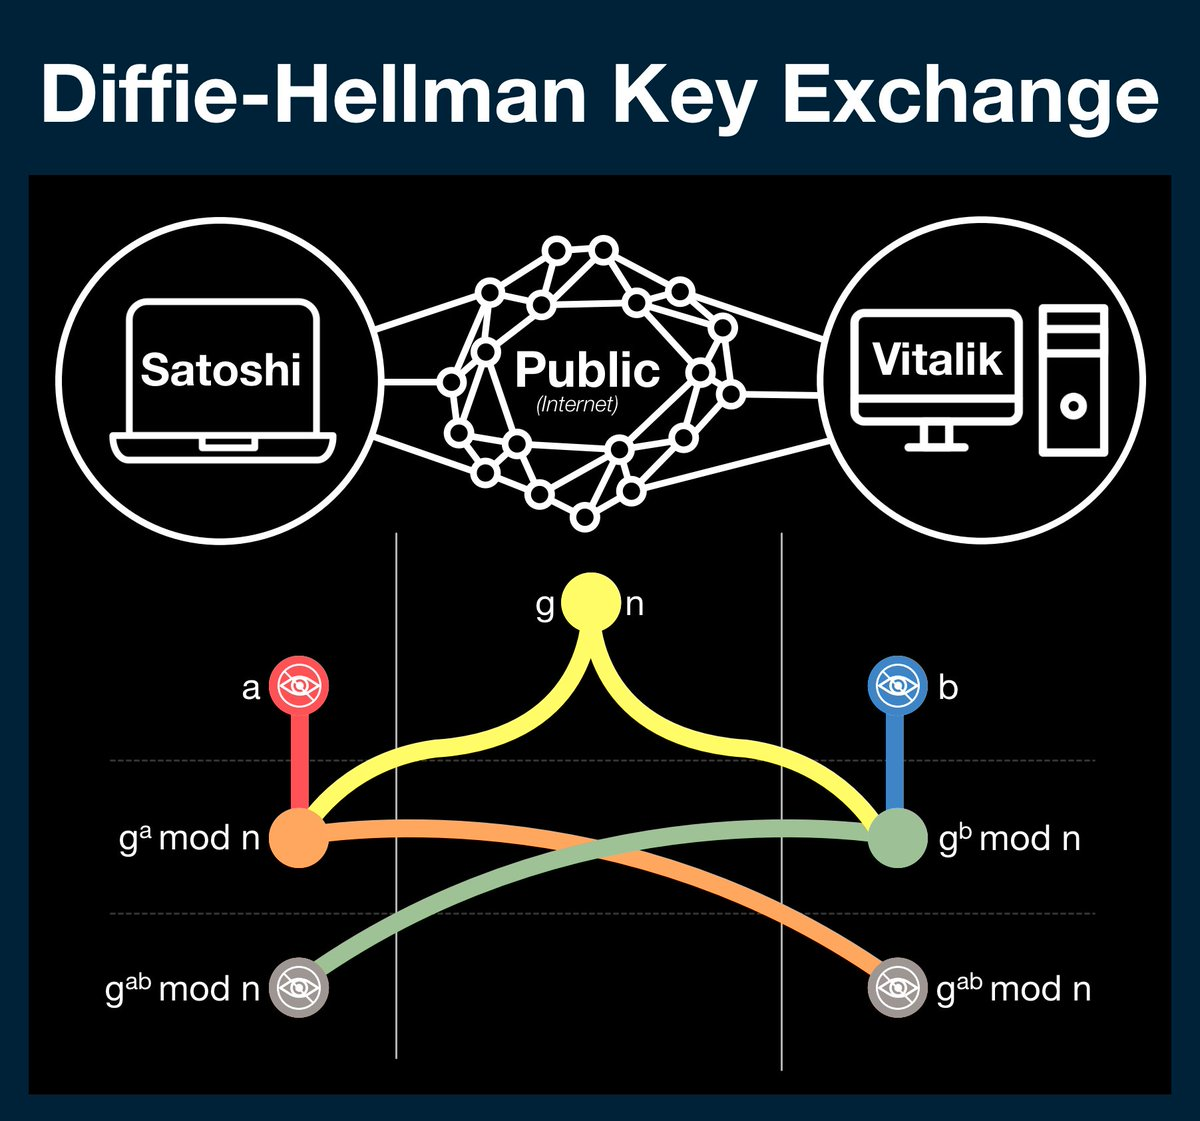
\includegraphics[width=1\textwidth]{\FIGURES/diffie-hellman-1.jpeg}
    \caption{Schéma Diffie-Hellmanova protokolu. Zdroj: \parencite{diffie-hellman-1}}
    \label{fig:diffie-hellman}
  \end{figure}

\newpage